\documentclass[floatsintext,mask,man]{apa6}

\usepackage{amssymb,amsmath}
\usepackage{ifxetex,ifluatex}
\usepackage{fixltx2e} % provides \textsubscript
\ifnum 0\ifxetex 1\fi\ifluatex 1\fi=0 % if pdftex
  \usepackage[T1]{fontenc}
  \usepackage[utf8]{inputenc}
\else % if luatex or xelatex
  \ifxetex
    \usepackage{mathspec}
    \usepackage{xltxtra,xunicode}
  \else
    \usepackage{fontspec}
  \fi
  \defaultfontfeatures{Mapping=tex-text,Scale=MatchLowercase}
  \newcommand{\euro}{€}
\fi
% use upquote if available, for straight quotes in verbatim environments
\IfFileExists{upquote.sty}{\usepackage{upquote}}{}
% use microtype if available
\IfFileExists{microtype.sty}{\usepackage{microtype}}{}

% Table formatting
\usepackage{longtable, booktabs}
\usepackage{lscape}
% \usepackage[counterclockwise]{rotating}   % Landscape page setup for large tables
\usepackage{multirow}		% Table styling
\usepackage{tabularx}		% Control Column width
\usepackage[flushleft]{threeparttable}	% Allows for three part tables with a specified notes section
\usepackage{threeparttablex}            % Lets threeparttable work with longtable

% Create new environments so endfloat can handle them
% \newenvironment{ltable}
%   {\begin{landscape}\begin{center}\begin{threeparttable}}
%   {\end{threeparttable}\end{center}\end{landscape}}

\newenvironment{lltable}
  {\begin{landscape}\begin{center}\begin{ThreePartTable}}
  {\end{ThreePartTable}\end{center}\end{landscape}}




% The following enables adjusting longtable caption width to table width
% Solution found at http://golatex.de/longtable-mit-caption-so-breit-wie-die-tabelle-t15767.html
\makeatletter
\newcommand\LastLTentrywidth{1em}
\newlength\longtablewidth
\setlength{\longtablewidth}{1in}
\newcommand\getlongtablewidth{%
 \begingroup
  \ifcsname LT@\roman{LT@tables}\endcsname
  \global\longtablewidth=0pt
  \renewcommand\LT@entry[2]{\global\advance\longtablewidth by ##2\relax\gdef\LastLTentrywidth{##2}}%
  \@nameuse{LT@\roman{LT@tables}}%
  \fi
\endgroup}


  \usepackage{graphicx}
  \makeatletter
  \def\maxwidth{\ifdim\Gin@nat@width>\linewidth\linewidth\else\Gin@nat@width\fi}
  \def\maxheight{\ifdim\Gin@nat@height>\textheight\textheight\else\Gin@nat@height\fi}
  \makeatother
  % Scale images if necessary, so that they will not overflow the page
  % margins by default, and it is still possible to overwrite the defaults
  % using explicit options in \includegraphics[width, height, ...]{}
  \setkeys{Gin}{width=\maxwidth,height=\maxheight,keepaspectratio}
\ifxetex
  \usepackage[setpagesize=false, % page size defined by xetex
              unicode=false, % unicode breaks when used with xetex
              xetex]{hyperref}
\else
  \usepackage[unicode=true]{hyperref}
\fi
\hypersetup{breaklinks=true,
            pdfauthor={},
            pdftitle={An Econometric Analysis of the Factors playing into gun violence within the United States},
            colorlinks=true,
            citecolor=blue,
            urlcolor=blue,
            linkcolor=black,
            pdfborder={0 0 0}}
\urlstyle{same}  % don't use monospace font for urls

\setlength{\parindent}{0pt}
%\setlength{\parskip}{0pt plus 0pt minus 0pt}

\setlength{\emergencystretch}{3em}  % prevent overfull lines


% Manuscript styling
\captionsetup{font=singlespacing,justification=justified}
\usepackage{csquotes}
\usepackage{upgreek}

 % Line numbering
  \usepackage{lineno}
  \linenumbers


\usepackage{tikz} % Variable definition to generate author note

% fix for \tightlist problem in pandoc 1.14
\providecommand{\tightlist}{%
  \setlength{\itemsep}{0pt}\setlength{\parskip}{0pt}}

% Essential manuscript parts
  \title{An Econometric Analysis of the Factors playing into gun violence within
the United States}

  \shorttitle{Gun Violence in the United States}


  \author{Kyle Vokes\textsuperscript{1}}

  % \def\affdep{{""}}%
  % \def\affcity{{""}}%

  \affiliation{
    \vspace{0.5cm}
          \textsuperscript{1} Macewan University  }

  \authornote{
    Add complete departmental affiliations for each author here. Each new
    line herein must be indented, like this line.
    
    Enter author note here.
    
    Correspondence concerning this article should be addressed to Kyle
    Vokes, Postal address. E-mail:
    \href{mailto:kyle5432@gmail.com}{\nolinkurl{kyle5432@gmail.com}}
  }


  \abstract{This study seeks to establish a casual relationship between gun
ownership and gun crime, in a manner that can be extrapolated to overall
levels of murder. The study found a strong correlation}
  \keywords{keywords \\

    \indent Word count: X
  }





\usepackage{amsthm}
\newtheorem{theorem}{Theorem}[section]
\newtheorem{lemma}{Lemma}[section]
\theoremstyle{definition}
\newtheorem{definition}{Definition}[section]
\newtheorem{corollary}{Corollary}[section]
\newtheorem{proposition}{Proposition}[section]
\theoremstyle{definition}
\newtheorem{example}{Example}[section]
\theoremstyle{definition}
\newtheorem{exercise}{Exercise}[section]
\theoremstyle{remark}
\newtheorem*{remark}{Remark}
\newtheorem*{solution}{Solution}
\begin{document}

\maketitle

\setcounter{secnumdepth}{0}



\subsection{Introduction}\label{introduction}

Violent crime within the United States is a very poignant issue at this
point in time, and one that represents a ripe area for econometric
study. Of key note, despite an environment which may very easily lead
one to believe the contrary, gun crime within the United States has
actually declined significantly over the last 40 years. This fact alone
can help omit numerous claims often made by the media, such as blaming
violent video games (these became prevalent right around the same time
crime rates started dropping). This highlights socio-economic factors,
as well as gun prevalence as a more likely cause. Within this study, it
is sought to develop a model that explains the interstate variation in
homicide, and explore the connection between firearm ownership rates and
firearm homicide rates. It is also worth noting that overall murder
rates and firearm murder rates are almost collinear, with an \(R^2\) of
0.85 for a simple model regressing the former on the later. This means
that whilst the firearm homicide rate is used as the dependent variable
within this study, the results can be quite accurately extrapolated to
overall murder rates as well.

\begin{figure}
\centering
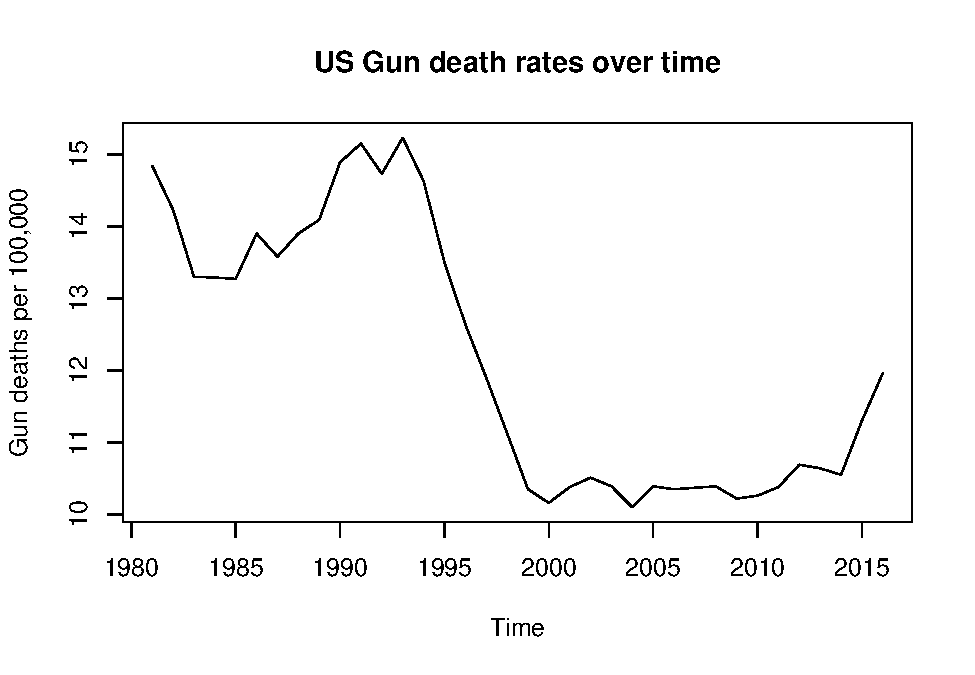
\includegraphics{as_files/figure-latex/unnamed-chunk-2-1.pdf}
\caption{}
\end{figure}

\subsection{Literacture Review}\label{literacture-review}

The topic of gun violence and murder has been a keystone topic within
the United States for decades. Contrasted with developed countries of
similar levels of economic development, the United States has a murder
rate several times higher than average. Siegel, Ross, and King (2013)
provides an excellent overview of the relationship between gun violence
and gun ownership. Using panel data from 1981 to 2010, firearm ownership
is found to be a strong indicator of gun homicide (incidence rate
ratio=1.009). This study also suggests the usage of age-adjusted
homicide rates over generic homicide rates, which proved crucial in
finding an accurate predictor.

Webster et. al. (2012) provides an excellent overview of current firearm
laws across the United States, which proved invaluable in putting
together binary variables to test the efficacy of various gun control
measures. Along with this, the study provides a good oversight of the
current climate surrounding gun ownership restrictions within the United
States.

Colonescu (2016) gave an excellent overview of all econometric methods
relevant to the research performed. The diagnostic

One more shit goes here

\subsection{Methodology \& Data}\label{methodology-data}

\subsubsection{Methodology}\label{methodology}

For this study, murder rates and gun ownership levels are hypothesized
to have a positive correlation. In order to show this, we must show a
statistically significant correlation between crime and gun ownership
levels even when socioeconomic factors are properly controlled for. This
would run contrary to the logic stated by the NRA and other guns-rights
movements within the United States that an increased presence of guns
serves to deter crime.

\subsubsection{Data}\label{data}

One of the key objectives when compiling the data set was to properly
minimize omitted variable bias. Crime is a complex and multifaceted
problem with many factors leading into it, so great care was taken to
properly control for any relevant socio-economic factors, particularly
those identified within the literature review. The data set includes the
variable poverty, which is the percentage of population within a state
living below the poverty line. The variable educ gives the number of
people within a state who have attained at least a bachelors degree. The
data for both of these variables came from the United States Census
Bureau.

~

\begin{tabular}{l|r|r|r|r|r}
\hline
  & gun & border & poverty & education & divorce\\
\hline
median & 32.250000 & 40.6366667 & 14.8000000 & 28.2000000 & 3.7000000\\
\hline
mean & 33.086000 & 38.2455258 & 14.8020000 & 29.0120000 & 3.7560000\\
\hline
SE.mean & 1.912592 & 1.3470657 & 0.4339895 & 0.6977786 & 0.1142200\\
\hline
CI.mean.0.95 & 3.843498 & 2.7099467 & 0.8721345 & 1.4022387 & 0.2295336\\
\hline
var & 182.900412 & 87.1001288 & 9.4173429 & 24.3447510 & 0.6523102\\
\hline
std.dev & 13.524068 & 9.3327450 & 3.0687689 & 4.9340400 & 0.8076572\\
\hline
coef.var & 0.408755 & 0.2440219 & 0.2073212 & 0.1700689 & 0.2150312\\
\hline
\end{tabular}

Table 2: Descriptive Statistics

In addition to socio-economic factors, one also must consider the
effects of availability of guns in neighboring states. If a state has
extremely strict gun laws, but an individual can easily travel to a
different state to circumvent these laws, this must be captured in the
data. In order to do so, an index was created via the formula below.
This gives a rough measure of the ease of circumventing local gun laws
and restrictions.

\begin{center}
$B^i=\frac{\sum G^{b}}{B}$ 
\end{center}

\(G^{b}\) = Gun ownership of bordering states\\
B = Number of bordering states

~

In order to conduct our multiple linear regression analysis, it must be
ensured that the data meets the Gauss-Markov assumptions. The first
assumption, the linearity of parametres, is met as the regression is in
the form:

\begin{center}
    $y=\beta _{0} +\beta _{2} x_{1}+ \beta_{2}x_{2} + ...+u$
    \end{center}

The second assumption of random sampling is almost entirely met. The
data used is almost entirely complete, aside from extrapolated marriage
data for California, and the border index having two. For the third
assumption to be met, we cannot have complete collinearity and no
variable may be constant.Table 3 confirms these assumptions are met.
Finally, the assumption of homoscedasticity is confirmed through the
Breusch-Pagan test.\\

\begin{center}
Table 3: Correlation Matrix
\end{center}

\begin{tabular}{l|l|l|l|l|l|l}
\hline
  & agemurder & gunrate & borderchainav & poverty & educ & divorce\\
\hline
Age-Adjusted Firearm Homocide & 1 &  &  &  &  & \\
\hline
Gun ownership & 0.69 & 1 &  &  &  & \\
\hline
Border Chain Index & 0.56 & 0.69 & 1 &  &  & \\
\hline
Poverty Rate & 0.56 & 0.32 & 0.14 & 1 &  & \\
\hline
Educational Attainment & -0.72 & -0.59 & -0.42 & -0.7 & 1 & \\
\hline
Divorce Rate & 0.64 & 0.51 & 0.33 & 0.35 & -0.54 & 1\\
\hline
\end{tabular}

\subsection{Results \& Analysis}\label{results-analysis}

For our initial benchmark model, we will use age-adjusted murder rate as
the independent variable, and percentage of households owning guns as
the dependent variable. It is worth noting that no correlation exists
without using the age-adjusted rate, suggesting demographic shape plays
a significant role in crime determination. Our baseline case shows a
strong correlation with gun ownership rates and age-adjusted homicide
rates, this is displayed in Figure \#, and the relationship given by the
formula below:

\begin{center}
    $\widehat{murder} = 4.68847 + 0.212*\mathit{gunrate}$
    \end{center}

\begin{figure}
\centering
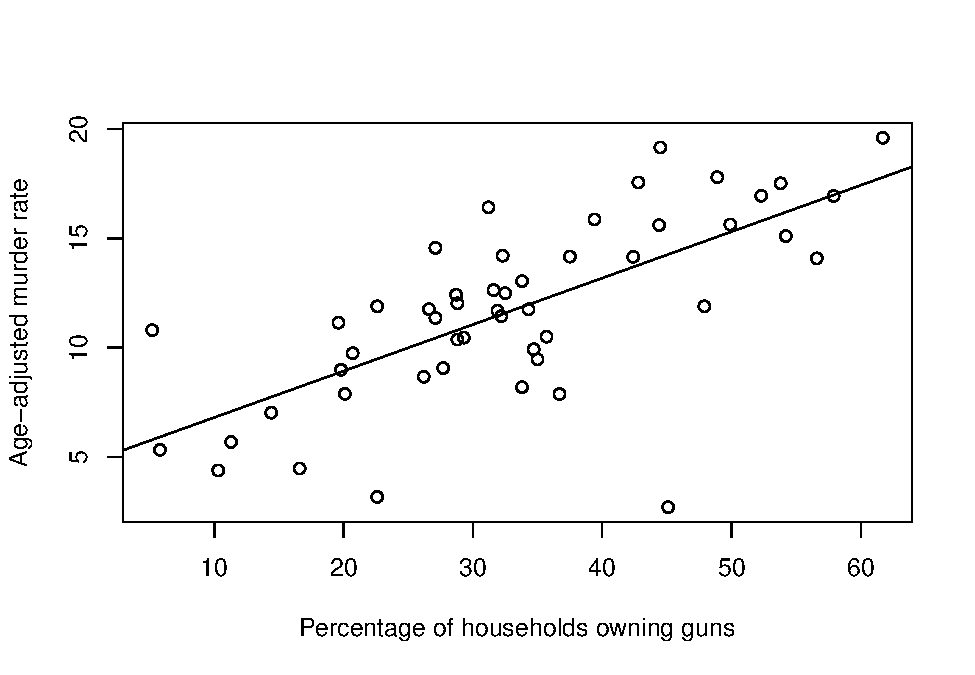
\includegraphics{as_files/figure-latex/unnamed-chunk-7-1.pdf}
\caption{}
\end{figure}

From here,the model will be refined by adding further independent
variables in order to control for socio-economic factors. The first
additional variable included was the poverty rate, which in itself is a
strong predictor of crime. It is worth noting that from here the
intercept coffecient ceases to be significant; also that controlling for
poverty causes reduction of 0.037 murders per 1\% increase in households
owning guns. The overall relationship is given by the formula below:

\begin{center}
$\widehat{murder} = -1.606 + 0.17535*\mathit{gunrate} + 0.50771*\mathit{poverty}$
\end{center}

The percentage of households owning guns serves to a reasonable degree
to capture the degree of gun control measures enacted within a state.
However, given the lax nature of interstate border enforcement, the ease
circumventing local laws must also be accounted for within the model.
This is done via the border chain index variable. The additional of this
control presents an interesting finding in of itself; the effect of a
1\% higher gun ownership per capita in neighbouring states has only
around half the impact on a states homocide rate as a 1\% increase of
ownership in the state itself. The overall relationship in this model is
given below:\\

\begin{center}
$\widehat{murder} = -2.918 + 0.140*\mathit{gunrate} + 0.480*\mathit{poverty} + 0.0772*\mathit{borderchainav}$
\end{center}

Educational attainment also serves as a strong predictor of overall
crime, and captures a number of factors we should wish to control for.
As expected, education has a negative overall impact on murder rates,
and the inclution of this control sees the impact of gun ownership
decline slightly over the previous model. As usual, the relationship
given by this model is given in the formula below:

\begin{center}
$\widehat{murder} = -2.918 + 0.140*\mathit{gunrate} + 0.480*\mathit{poverty} + 0.0772*\mathit{borderchainav} + -0.250*\mathit{educ}$
\end{center}

The final control variable used was the per capita divorce rate for each
state. This captures a number of key factors should be controlled for,
such as the stability of home life during childhood. It is worth noting
that within the American political arena, decline in family values is
often blamed for gun violence. This is only a half truth, as the overall
divorce rate has been steadily dropping for several decades within the
United States. However, the final model did find divorce rates to be a
strong predicter of homicide rates.

\begin{tabular}{l|c|c|c|c}
\hline
  & Estimate & Std. Error & t & p-Value\\
\hline
(Intercept) & 3.760 & 5.385 & 0.698 & 0.489\\
\hline
gunrate & 0.090 & 0.033 & 2.721 & 0.010\\
\hline
poverty & 0.230 & 0.132 & 1.737 & 0.090\\
\hline
borderchainav & 0.065 & 0.040 & 1.640 & 0.109\\
\hline
divorce & 1.148 & 0.418 & 2.748 & 0.009\\
\hline
educ & -0.178 & 0.097 & -1.838 & 0.074\\
\hline
\end{tabular}

\begin{verbatim}
## [1] "R²=0.7369"
\end{verbatim}

Additional inference can be drawn from lumping states with similar
levels of gun ownership together and finding factors that lead to
differences between these groups. With this procedure, 3 different
groups have been created. Alabama, Arkansas, Idaho, Montana, and West
Virginia, South Dakota all have rates of gun ownership in the mid 50s
yet considerable variance is seen in crime rates between our states. The
second group is comprised of Hawaii and the District of Columbia. Both
of these states have next to no gun ownership, yet have a massive
disparity in

\begin{figure}
\centering
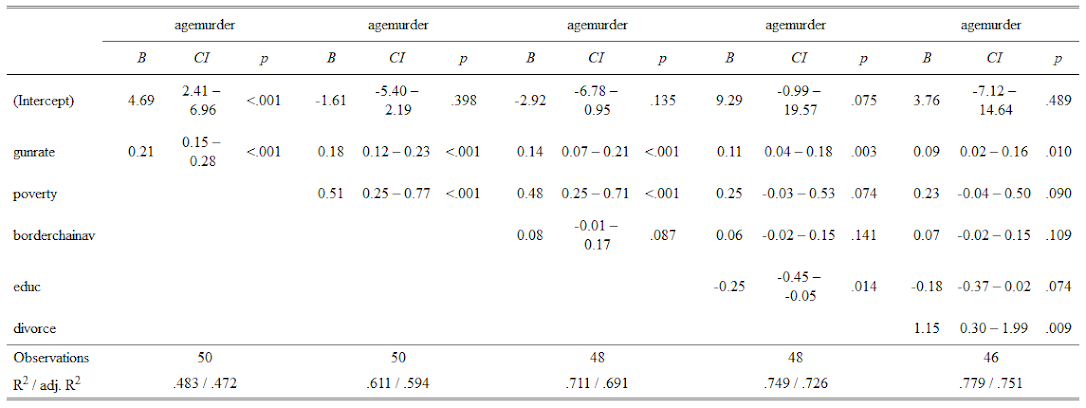
\includegraphics{C:/Users/Kyle/Documents/399 project/regression.png}
\caption{Comparison of regression models}
\end{figure}

\section{Conclusion}\label{conclusion}

Overall, this paper finds gun ownership per capita to be a significant
factor in explaining the large variation of overall level of homicide
between US states. Within the final model, a 1\% increase in households
owning firearms causes an increase in the per capita homicide rate by

\newpage

\section{References}\label{references}

\begingroup
\setlength{\parindent}{-0.5in} \setlength{\leftskip}{0.5in}

\hypertarget{refs}{}

\endgroup

\newpage

\section{Appendix}\label{appendix}

A.1 Details of Variables Used Within Model

\begin{longtable}[]{@{}lllll@{}}
\toprule
\begin{minipage}[b]{0.29\columnwidth}\raggedright\strut
Full Name\strut
\end{minipage} & \begin{minipage}[b]{0.09\columnwidth}\raggedright\strut
Model Name\strut
\end{minipage} & \begin{minipage}[b]{0.22\columnwidth}\raggedright\strut
Source\strut
\end{minipage} & \begin{minipage}[b]{0.22\columnwidth}\raggedright\strut
Comments\strut
\end{minipage} & \begin{minipage}[b]{0.04\columnwidth}\raggedright\strut
Link\strut
\end{minipage}\tabularnewline
\midrule
\endhead
\begin{minipage}[t]{0.29\columnwidth}\raggedright\strut
Age-Adjusted Firearm Death Rates\strut
\end{minipage} & \begin{minipage}[t]{0.09\columnwidth}\raggedright\strut
agemurder\strut
\end{minipage} & \begin{minipage}[t]{0.22\columnwidth}\raggedright\strut
CDC Center for Health Statistics\strut
\end{minipage} & \begin{minipage}[t]{0.22\columnwidth}\raggedright\strut
Complete for all states, 2014\strut
\end{minipage} & \begin{minipage}[t]{0.04\columnwidth}\raggedright\strut
\href{https://www.cdc.gov/nchs/pressroom/sosmap/firearm.htm}{1}\strut
\end{minipage}\tabularnewline
\begin{minipage}[t]{0.29\columnwidth}\raggedright\strut
Percentage of Households Owning Firearms\strut
\end{minipage} & \begin{minipage}[t]{0.09\columnwidth}\raggedright\strut
gunrate\strut
\end{minipage} & \begin{minipage}[t]{0.22\columnwidth}\raggedright\strut
Gun Ownership \& Social Gun Culture\strut
\end{minipage} & \begin{minipage}[t]{0.22\columnwidth}\raggedright\strut
Complete for all states, 2013\strut
\end{minipage} & \begin{minipage}[t]{0.04\columnwidth}\raggedright\strut
\href{http://injuryprevention.bmj.com/content/injuryprev/early/2015/06/09/injuryprev-2015-041586.full.pdf?keytype=ref\&ijkey=doj6vx0laFZMsQ2}{2}\strut
\end{minipage}\tabularnewline
\begin{minipage}[t]{0.29\columnwidth}\raggedright\strut
Poverty Rate by Household Income\strut
\end{minipage} & \begin{minipage}[t]{0.09\columnwidth}\raggedright\strut
poverty\strut
\end{minipage} & \begin{minipage}[t]{0.22\columnwidth}\raggedright\strut
United States Census Bureau\strut
\end{minipage} & \begin{minipage}[t]{0.22\columnwidth}\raggedright\strut
Complete for all states, 2014\strut
\end{minipage} & \begin{minipage}[t]{0.04\columnwidth}\raggedright\strut
\href{https://www.census.gov/content/dam/Census/library/publications/2015/demo/p60-252.pdf}{3}\strut
\end{minipage}\tabularnewline
\begin{minipage}[t]{0.29\columnwidth}\raggedright\strut
Divorces per 1,000\strut
\end{minipage} & \begin{minipage}[t]{0.09\columnwidth}\raggedright\strut
divorce\strut
\end{minipage} & \begin{minipage}[t]{0.22\columnwidth}\raggedright\strut
CDC Center for Health Statistics\strut
\end{minipage} & \begin{minipage}[t]{0.22\columnwidth}\raggedright\strut
Indiana and Louisiana missing, 2011\strut
\end{minipage} & \begin{minipage}[t]{0.04\columnwidth}\raggedright\strut
\href{https://www.cdc.gov/nchs/data/dvs/divorce_rates_90_95_99-11.pdf}{4}\strut
\end{minipage}\tabularnewline
\begin{minipage}[t]{0.29\columnwidth}\raggedright\strut
Percentage of Residents With Bachelors or Higher\strut
\end{minipage} & \begin{minipage}[t]{0.09\columnwidth}\raggedright\strut
educ\strut
\end{minipage} & \begin{minipage}[t]{0.22\columnwidth}\raggedright\strut
United States Census Bureau\strut
\end{minipage} & \begin{minipage}[t]{0.22\columnwidth}\raggedright\strut
Complete for all states, 2014\strut
\end{minipage} & \begin{minipage}[t]{0.04\columnwidth}\raggedright\strut
\href{https://factfinder.census.gov/faces/tableservices/jsf/pages/productview.xhtml?pid=ACS_15_5YR_S1501}{5}\strut
\end{minipage}\tabularnewline
\begin{minipage}[t]{0.29\columnwidth}\raggedright\strut
Average Gun Ownership of Neighbouring States\strut
\end{minipage} & \begin{minipage}[t]{0.09\columnwidth}\raggedright\strut
borderchainav\strut
\end{minipage} & \begin{minipage}[t]{0.22\columnwidth}\raggedright\strut
Self Created Index\strut
\end{minipage} & \begin{minipage}[t]{0.22\columnwidth}\raggedright\strut
Null entry for Hawaii and Alaska\strut
\end{minipage} & \begin{minipage}[t]{0.04\columnwidth}\raggedright\strut
NA\strut
\end{minipage}\tabularnewline
\bottomrule
\end{longtable}

~

~

agemurder

~

agemurder

~

~

B

CI

p

~

B

CI

p

(Intercept)

~

4.69

2.41~--~6.96

\textless{}.001

~

-1.61

-5.40~--~2.19

.398

gunrate

~

0.21

0.15~--~0.28

\textless{}.001

~

0.18

0.12~--~0.23

\textless{}.001

poverty

~

~

~

0.51

0.25~--~0.77

\textless{}.001

Observations

~

50

~

50

R2 / adj. R2

~

.483 / .472

~

.611 / .594






\end{document}
